% !TEX encoding = UTF-8 Unicode
\documentclass[11pt]{beamer}
\usepackage{luatexja}
\usepackage[haranoaji,deluxe]{luatexja-preset}
\usepackage{amsmath}
\usepackage{amsthm}
\setbeamertemplate{proof begin}{\noindent\textbf{証明}\quad}
\setbeamertemplate{proof end}{\qed \par}
\setbeamertemplate{bibliography item}[text]

\theoremstyle{plain}
\newtheorem{thm}{定理}
\newtheorem*{thm*}{定理}
\newtheorem{cor}{系}
\newtheorem{lem}{補題}
\newtheorem{assumption}{仮定}

\theoremstyle{definition}
\newtheorem{dfn}{定義}
\def\qedsymbol{}
% ------------------------------
%  pLaTeX で日本語を扱う設定例
% ------------------------------
% hyperref で日本語 PDF しおり等が化けないように

% 数式や画像，色の設定
\usepackage{amsmath,amssymb}
\usepackage{graphicx}
\usepackage{xcolor}
\usepackage{array}
\usepackage[authoryear,round]{natbib}
\bibpunct{(}{)}{;}{a}{ }{,}
\let\oldcite\cite
\renewcommand{\cite}[1]{\citealp{#1}}
\newcommand{\E}{\mathbb{E}}
\newcommand{\Tr}{\operatorname{Tr}}

% ------------------------------
% Beamer のテーマや色の設定
% ------------------------------
\usetheme{Madrid}       % お好みのテーマに変更可能
\usecolortheme{beaver}  % 赤系配色の例

% スライド下部にページ番号を表示したい場合
\setbeamertemplate{footline}[frame number]
% ナビゲーションアイコンを消す場合
\setbeamertemplate{navigation symbols}{}
\usepackage{tikz}
\usetikzlibrary{positioning, arrows.meta, calc}


% for hyperref
\hypersetup{
	colorlinks=true, % リンクに色をつけない設定
	bookmarks=true, % 以下ブックマークに関する設定
	bookmarksnumbered=true,
	pdfborder={0 0 0},
	bookmarkstype=toc
}

% ------------------------------
% タイトル情報
% ------------------------------
\title{データの内在次元を用いた拡散モデルの収束解析}
%\subtitle{}
\author{枇榔 一真}
\institute{深澤研究室 M2}
\date{2026年8月20日}

% ------------------------------
\begin{document}

% =====================================================================
% PDFページ対応表（現在のビルド: 全44ページ）
% 各frameの直前に「Frame番号 | PDFページ | 内容」を記載している。
% 参考文献のframeのみ allowframebreaks によりPDF 36--44ページに分割される。
% frameの追加・削除や参考文献の増減後は、このページ表記も更新すること。
% =====================================================================

% ===== Frame 01 | PDF p.01 | タイトル =====
\begin{frame}
  \titlepage
\end{frame}

% ===== Frame 02 | PDF p.02 | 目次 =====
  \begin{frame}{目次}
    \begin{itemize}
      \item 拡散モデルは, 画像生成, 動画生成, タンパク質の構造生成など, データの生成を行うことのできるアルゴリズムであり, 近年機械学習で盛んに研究が行われている.
      \item そのアルゴリズムは確率微分方程式(SDE)でモデル化することができる. 本発表では, 拡散モデルの収束解析という確率微分方程式の評価をする問題として定式化された問題について紹介する.
    \end{itemize}
    \begin{block}{発表の流れ}
    \begin{enumerate}
      \item 拡散モデルについて
      \item 拡散モデルの収束解析について
      \item 研究結果
      \item 証明概要
    \end{enumerate}
    \end{block}
  \end{frame}

% % ===== 無効化済み | 旧 PDF p.03 | NeurIPS 2024における拡散モデル研究 =====
% \begin{frame}{拡散モデルについて}
%   \begin{itemize}
%     \item 拡散モデルは近年機械学習の分野で盛んに研究されている手法である.
%     \item 機械学習のトップ会議 NeurIps 2024では, 大規模言語モデルの次に研究数が多かったのが拡散モデルである.
%   \end{itemize}
%   \vspace{0.1cm}
%   \begin{center}
%     \includegraphics[width=0.86\textwidth,height=0.68\textheight,keepaspectratio]{top_topics_2024.png}\\[-0.15cm]
%     {\tiny
%       Shayan Mousavi,
%       \href{https://shmouses.github.io/NeurIPS2024AITrends/}{NeurIPS 2024 AI Research Trends}
%     }
%   \end{center}
% \end{frame}

% ===== Frame 03 | PDF p.03 | 生成とは =====
  \begin{frame}{拡散モデルについて : 生成とは}
    \begin{block}{拡散モデルの目的}
      未知の確率測度 $P_{\text{data}}$ に従って独立に得られたデータ $\{x_1,\cdots, x_n\}\subset \mathbb{R}^d$ があるとする.

      このデータを用いて, $P_{\text{data}}$ に従う新たなデータを近似的に生み出すことを\textcolor{red}{生成}という.
      \begin{center}
    \begin{tikzpicture}[
      node distance=2.2cm,
      box/.style={
        draw,
        rounded corners,
        minimum width=3.0cm,
        minimum height=1.3cm,
        align=center
      },
      arrow/.style={
        -{Latex[length=3mm]},
        thick
      }
    ]
    
    \node[box] (data) {
      $x_1,\ldots,x_n \sim P_{\text{data}}$\\
      \small 既存のデータ
    };
    
    \node[box, right=of data] (model) {
      $x_{\text{new}}\sim \widehat{P}\approx P_{\text{data}}$\\
      \small 新たなデータを生成
    };
    
    \draw[arrow] (data) -- node[above] {\small } (model);

    \end{tikzpicture}
    \end{center}
    \end{block}
    \begin{block}{生成モデル}
      生成を行う機械学習のモデルを, \textcolor{red}{生成モデル} という.
      \par
      \centering
      \begin{tikzpicture}[
        category/.style={
          draw,
          rounded corners=2pt,
          minimum width=2.5cm,
          minimum height=0.64cm,
          align=center,
          font=\small
        },
        modeltype/.style={
          draw,
          rounded corners=2pt,
          minimum width=2.7cm,
          minimum height=0.52cm,
          align=center,
          font=\small
        },
        branch/.style={thick}
      ]
        \node[category] (generative) {生成モデル};
        \node[modeltype, right=2.2cm of generative, yshift=0.61cm] (vae) {VAE};
        \node[modeltype, right=2.2cm of generative] (gan) {GAN};
        \node[modeltype, right=2.2cm of generative, yshift=-0.61cm] (diffusion) {\textcolor{red}{拡散モデル}};

        \coordinate (fork) at ($(generative.east)+(0.9cm,0)$);
        \draw[branch] (generative.east) -- (fork);
        \draw[branch] (fork) |- (vae.west);
        \draw[branch] (fork) -- (gan.west);
        \draw[branch] (fork) |- (diffusion.west);
      \end{tikzpicture}
    \end{block}
  \end{frame}
% ===== Frame 04 | PDF p.04 | 拡散モデルの原理 =====
  \begin{frame}{拡散モデルについて : SDEを用いた生成}
    $\{W_t\}_{t\in[0,T]}$ をブラウン運動として, 次のSDEを考える.
    \begin{align*}
        dY_t=b(t,Y_t)dt+\sigma(t,Y_t)dW_t\quad (t\in[0,T])
    \end{align*}
    上記のSDEの解 $\{Y_t\}_{t\in[0,T]}$ が次の2つの性質を満たすように, $b$ と $\sigma$ を設計できるかということを考える.
    \begin{enumerate}
      \item 初期分布 $\mathcal{L}(Y_0)$ が, 容易にサンプルが得られる分布である (正規分布, 一様分布など)
      \item 最終時刻の分布が $P_{\text{data}}$ と等しい. つまり, $\mathcal{L}(Y_T)=P_{\text{data}}$ .
    \end{enumerate}

    \vspace{0.15cm}
    \begin{center}
    \begin{tikzpicture}[
      node distance=5.2cm,
      box/.style={
        draw,
        rounded corners,
        minimum width=2.8cm,
        minimum height=1.15cm,
        align=center
      },
      arrow/.style={
        -{Latex[length=3mm]},
        thick
      }
    ]

    \node[box] (normal) {
      $Y_0$\\
      \small サンプルが容易な分布
    };

    \node[box, right=of normal] (data) {
      $Y_T\sim P_{\text{data}}$\\
      \small データ分布
    };

    \draw[arrow] (normal) -- node[above] {\small $dY_t=b(t,Y_t)dt+\sigma(t,Y_t)dW_t$} (data);

    \end{tikzpicture}
    \end{center}
  \end{frame}
  \begin{frame}{拡散モデルについて : Ornstein Uhlenbeck process}
    \begin{block}{Ornstein Uhlenbeck process}
      次のSDEの解 $\{X_t\}_{t\in[0,T]}$ をOrnstein–Uhlenbeck processという.
      \begin{equation*}
        dX_t=-X_tdt+\sqrt{2}dW_t \quad (t\in[0,T])
      \end{equation*}
    \end{block}
      Ornstein–Uhlenbeck processは明示的に解くことができ, $X_0$ と独立な標準正規分布に従う確率変数 $Z$ が存在して, 
      \begin{equation*}
        X_t=e^{-t}X_0+\sqrt{2}\int_{0}^{t}e^{-(t-s)}dW_s=e^{-t}X_0+\sqrt{1-e^{-2t}}Z
      \end{equation*}
      と書ける. これにより, $T$ を十分大きくとると $X_T$ の分布は標準正規分布 $\mathcal{N}(0,I_d)$ に近づいていく.

      $\mathcal{L}(X_0)=P_{\text{data}}$ とすると, $X$ は $P_\text{data}$ から時間経過とともに
      $\mathcal{N}(0,I)$ へ近づいていく過程とみなせる.
    \begin{center}
    \begin{tikzpicture}[
      node distance=5.2cm,
      box/.style={
        draw,
        rounded corners,
        minimum width=2.8cm,
        minimum height=1.15cm,
        align=center
      },
      arrow/.style={
        -{Latex[length=3mm]},
        thick
      }
    ]

    \node[box] (normal) {
      $\mathcal{L}(X_T)\approx \mathcal{N}(0,I_d)$
    };

    \node[box, right=of normal] (data) {
      $\mathcal{L}(X_0)= P_{\text{data}}$\\
      \small データ分布
    };

    \draw[arrow] (data) -- node[above] {\small $dX_t=-X_tdt+\sqrt{2}dW_t$} (normal);

    \end{tikzpicture}
    \end{center}

  \end{frame}
% ===== Frame 05 | PDF p.05 | 拡散過程の時間反転構造（導入） =====
  \begin{frame}{拡散モデルについて : 拡散過程の時間反転公式}
    $\{X_t\}_{t\in[0,T]}$ をOrnstein–Uhlenbeck processとして, $0<t\leqq T$ のとき, $X_t$ の密度を $p_t$ とする.
    \begin{theorem}[\cite{anderson82,haussmann_pardoux86}]
      $\{Y_t\}_{t\in[0,T]}$ を次のSDEの解とする.
      \begin{equation}
        \left\{ \,
            \begin{aligned}
            & dY_t = (Y_t+\nabla \log{p_{T-t}(Y_t)})dt+\sqrt{2}dW_t \quad (0< t < T) \\
            & Y_0 \stackrel{\mathrm{d}}{=} X_T
            \end{aligned}
        \right.
      \end{equation}
      このとき, 任意の $t\in[0,T]$ に対して, $Y_t\stackrel{\mathrm{d}}{=}X_{T-t}$ が成り立つ.
    \end{theorem}
    $\{X_t\}_{t\in[0,T]}$ の時間反転過程 $\{Y_t\}_{t\in[0,T]}$ は, $\mathcal{L}(X_T)\approx \mathcal{N}(0,I_d)$ から時間の経過とともに
        $P_{\text{data}}$ へ近づいていく確率過程となる.
    \begin{center}
    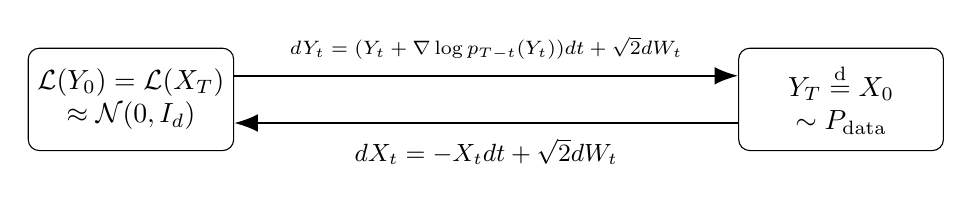
\begin{tikzpicture}[
      node distance=6.4cm,
      box/.style={
        draw,
        rounded corners,
        minimum width=2.6cm,
        minimum height=1.3cm,
        align=center
      },
      arrow/.style={
        -{Latex[length=3mm]},
        thick
      }
    ]

      \node[box] (normal) {
          $\mathcal{L}(Y_0)=\mathcal{L}(X_T)$\\
          $\approx \mathcal{N}(0,I_d)$
      };

    \node[box, right=of normal] (data) {
      $Y_T\stackrel{\mathrm{d}}{=}X_0$\\
      $\sim P_{\text{data}}$
    };

    \draw[arrow]
      ([yshift=0.30cm]normal.east) --
      node[above=2pt] {\scriptsize $dY_t=(Y_t+\nabla\log p_{T-t}(Y_t))dt+\sqrt{2}dW_t$}
      ([yshift=0.30cm]data.west);

    \draw[arrow]
      ([yshift=-0.30cm]data.west) --
      node[below=2pt] {\small $dX_t=-X_tdt+\sqrt{2}dW_t$}
      ([yshift=-0.30cm]normal.east);

    \end{tikzpicture}
    \end{center}
  \end{frame}


% ===== Frame 08 | PDF p.08 | 3つの誤差の発生源 =====
    \begin{frame}{拡散モデルについて : 3つの誤差の発生源}
    \begin{equation*}
        \left\{ \,
            \begin{aligned}
            & dY_t = (Y_t+\nabla \log{p_{T-t}(Y_t)})dt+\sqrt{2}dB_t \quad (0\leqq t \leqq T) \\
            & Y_0 \stackrel{\mathrm{d}}{=} X_T\approx \mathcal{N}(0,I_d)
            \end{aligned}
        \right.
    \end{equation*}
      上記のSDEをシミュレーションすると, $Y_T\sim P_{\text{data}}$ からのサンプリングが得られる. しかし, 現実的には以下の3つの点が問題となる.
      \begin{enumerate}
        \item 初期分布 $\mathcal{L}(X_T)$ からの厳密なサンプリングが得られない.
        \item スコア関数 $\nabla \log{p_{T-t}(Y_t)}$ が明示的に得られない.
        \item SDEを連続時間でシミュレーションできない.
      \end{enumerate}
      拡散モデルでは, それぞれの問題点に対して次のように対応する.
      \begin{enumerate}
        \item 初期分布を標準正規分布 $\mathcal{N}(0,I_d)$ にする.
        \item スコア関数を, $\nabla\log{p_{t}(y)}$ を, 推定量 $\hat{s}(t,y)$ に置き換える.
        \item 時間に関して離散化する.
      \end{enumerate}
  \end{frame}

  \begin{frame}{拡散モデルの収束解析について}
    \begin{itemize}
      \item 前頁のようにシミュレーションして得られるデータの分布を $\hat{P}_\text{data}$ とする.
      \item このとき, 確率測度の近さを測る指標 $\rho$ を用いて, $\rho(P_\text{data},\hat{P}_\text{data})$ を評価することを, 
    \textcolor{red}{拡散モデルの収束解析} と呼ぶ.
      \item 指標 $\rho$ として用いられるものは, 主に次の2種類である.
    {\large
      \begin{enumerate}
        \item Kullback-Leibler divergence
        \item 2-Wasserstein distance
      \end{enumerate}
    }
    \end{itemize}

  \end{frame}
% ===== Frame 11 | PDF p.11 | KLダイバージェンスの定義 =====
  {
    \setbeamerfont{frametitle}{size=\large}
    \begin{frame}{拡散モデルの収束解析について : Kullback-Leibler divergence}
      \small
      \footnotesize
      \begin{definition}
        2つの確率測度 $P, Q$ のKullback-Leibler divergence $D_{\text{KL}}(P|Q)$ を, 次のように定義する.
        \begin{equation*}
          D_{\text{KL}}(P\mid Q):=        \left\{ \,
            \begin{aligned}
            & \mathbb{E}_P\left[\log{\frac{dP}{dQ}}\right] \quad \bigl(P\ll Q\bigr) \\
            & \infty \quad \quad \quad\quad \quad \quad(\text{otherwise})
            \end{aligned}
        \right.
        \end{equation*}
      \end{definition}
      \small
      \vspace{-0.65em}
      \begin{theorem}[\cite{benton_et_al_2024}]
        ある定数 $C>0$ が存在して, 次の不等式が成立する.
        \vspace{-0.35em}
        \begin{equation*}
          D_{\mathrm{KL}}\bigl(P_{\text{data}}\mid \hat{P}_{\text{data}}\bigr)
          \leqq C\left(\underbrace{\frac{2dT^2}{N}}_{\text{離散化誤差}}+\underbrace{\epsilon_{\text{score}}}_{\text{スコア推定誤差}}+\underbrace{de^{-2T}}_{\text{初期分布誤差}}\right)
        \end{equation*}
        \vspace{-0.2em}
        \noindent
        $t_i=iT/N\quad(i=0,\ldots,N)$
        \par\vspace{0.25em}
        \noindent
        $\epsilon_{\text{score}}=(T/N)\sum\nolimits_{i=1}^{N}
          \mathbb{E}\!\left[
            \left\|\nabla\log p_{t_i}(X_{t_i})
            -\hat{s}(t_i,X_{t_i})\right\|^2
          \right]$
        \par\vspace{0em}
        \noindent{\scriptsize
          $N$: 時間離散化のステップ数\quad
          $d$: データの次元\quad
          $T$: SDEの終端時刻
        }
      \end{theorem}
  \end{frame}
  }
% ===== Restored frame | Wasserstein distance =====
  \begin{frame}{拡散モデルの収束解析について : Wasserstein distance}
    \small
    \begin{definition}
      $\mathbb{R}^d$上の確率測度$P,Q$に対して,
      $\Pi(P,Q)=\{\pi\text{ : }\mathbb{R}^d\times\mathbb{R}^d\text{上の確率測度}
      \mid\pi(\cdot,\mathbb{R}^d)=P,\pi(\mathbb{R}^d,\cdot)=Q\}$とする.
      このとき, $P,Q$の2-Wasserstein distance $W_2(P,Q)$を次のように定義する.
      \begin{equation*}
        W_2(P,Q)=\inf_{\pi\in\Pi(P,Q)}
        \left(\int_{\mathbb{R}^d\times\mathbb{R}^d}|x-y|^2d\pi(x,y)\right)^{\frac{1}{2}}.
      \end{equation*}
    \end{definition}
    \vspace{-0.4em}
    \begin{theorem}[\cite{koike_2026_wasserstein}, Theorem 3.3]
      $t_n=nT/N\ (n=0,\ldots,N)$ とする.
      正則性条件のもとで, ある定数
      $C_L>0$ が存在して, 次の不等式が成立する.
      \vspace{-0.4em}
      \begin{equation*}
        W_2\bigl(p_{\mathrm{data}},\mathcal{L}(\hat{Y}_{t_N})\bigr)
        \leqq C_L\Biggl(
          \underbrace{\frac{\sqrt{d}T}{N}}_{\text{離散化誤差}}
          +\underbrace{\sqrt{\epsilon_{\mathrm{score}}}}_{\text{スコア推定誤差}}
          +\underbrace{\sqrt{d}\,e^{-2T}}_{\text{初期分布誤差}}
        \Biggr).
      \end{equation*}
      \vspace{-0.2em}
      \noindent{\scriptsize
        $N$: 時間離散化のステップ数\quad
        $d$: データの次元\quad
        $T$: SDEの終端時刻
      }
    \end{theorem}
  \end{frame}
% ===== Frame 15 | PDF p.15 | データの内在次元に関する仮定 =====
  \begin{frame}{拡散モデルの収束解析について : データの内在次元}
    現実世界のデータ分布はごく少数の変数で記述されると考えられている. これは\textcolor{red}{多様体仮説}と呼ばれ, 機械学習の成功の基盤と考えられている (\cite{pope_et_al_2021}).
    \begin{center}
      \includegraphics[
        width=0.60\linewidth,
        trim=0 0 350bp 0,
        clip
      ]{\detokenize{スクリーンショット 2026-08-08 16.19.15.png}}
    \end{center}
    データ分布を記述する上で必要な変数の数を, データ分布の\textcolor{red}{内在次元} と呼ぶ.

    \cite{pope_et_al_2021} は, 代表的な画像のデータセットに対する内在次元推定を行い, 画像は $224\times 224 \times 3 = 15028$ の画素値を持つが, 内在次元は $26\sim 43$ 程度であるという結果を得ている.
  \end{frame}
% ===== Frame 16 | PDF p.12 | 次元と距離ごとの収束レート比較 =====
  \begin{frame}{拡散モデルの収束解析について : データの内在次元}
    データの次元 $d$ ではなく, 内在次元 $k$ を使った収束解析はKullback-Leibler divergence において行われており, 以下の結果が得られている.
    \begin{theorem}[\cite{huang_wei_chen_2026}]
      $t_n=nT/N\ (n=0,\ldots,N)$ とする.
      ある定数 $C>0$ が存在して, 次の不等式が成立する.
      \vspace{-0.5em}
      \begin{equation*}
        \begin{aligned}
          KL\left(P_{\text{data}}\mid\hat{P}_\text{data}\right)
          \leqq C\Biggl(&
          \underbrace{\frac{T^2}{N}k\log k}_{\text{離散化誤差}}
          +\underbrace{\epsilon_{\text{score}}}_{\text{スコア推定誤差}}
          +\underbrace{de^{-2T}}_{\text{初期分布誤差}}
          \Biggr).
        \end{aligned}
      \end{equation*}
      \vspace{-0.2em}
      \noindent{\scriptsize
        $N$: 時間離散化のステップ数\quad
        $d$: データの次元\quad
        $T$: SDEの終端時刻\quad
        $k$: 内在次元
      }
    \end{theorem}
  \end{frame}
% =====================================================================
% ここから（PDF p.18以降）を確率論の研究集会向けに再構成
% =====================================================================

% ===== Frame 17 | PDF p.13 | 次元と距離ごとの主結果比較 =====
\begin{frame}[t]{設定 : 主結果}
  \vspace{-0.65em}
  \centering
  \renewcommand{\arraystretch}{1.15}
  \setlength{\tabcolsep}{0.35em}
  \begin{tabular}{
    >{\centering\arraybackslash}m{0.08\textwidth}|
    >{\centering\arraybackslash}m{0.39\textwidth}|
    >{\centering\arraybackslash}m{0.42\textwidth}}
    \hline
    & {\large\textbf{KL divergence}}
    & {\large\textbf{2-Wasserstein distance}} \\
    \hline
    {\normalsize $d$次元}
    & {\footnotesize
      $\displaystyle
        \mathcal O\!\left(
          \frac{dT^2}{N}
          +\epsilon_{\mathrm{score}}
          +de^{-2T}
        \right)$
      \par\vspace{0.25em}
      {\scriptsize Benton et al. (2024)}}
    & {\footnotesize
      $\displaystyle
      \begin{aligned}
        \mathcal O\!\Bigg(&
          \frac{\sqrt d\,T}{N}
          +\sqrt{\epsilon_{\mathrm{score}}}+\sqrt d\,e^{-2T}
        \Bigg)
      \end{aligned}$
      \par\vspace{0.25em}
      {\scriptsize Koike (2026)}} \\
    \hline
    {\normalsize $k$次元}
    & {\footnotesize
      $\displaystyle
      \begin{aligned}
        \mathcal O\!\Bigg(&
          \frac{T^2}{N}k\log k
          +\epsilon_{\mathrm{score}}+de^{-2T}
        \Bigg)
      \end{aligned}$
      \par\vspace{0.25em}
      {\scriptsize Huang et al. (2026)}}
    & {\footnotesize
      \textcolor{red}{$\displaystyle
      \begin{aligned}
        \mathcal O\!\Bigg(&
        e^{T+\frac{2T}{N}\sum_{i=0}^{N-1}L(T-t_i)}
        \Bigg[\\[-0.1em]
        &T\sqrt{\frac{k\log k}{N}}+\varepsilon\\[-0.1em]
        &+e^{-T}\sqrt{M_2}+e^{-2T}\sqrt d
        \Bigg]\Bigg)
      \end{aligned}$}
      \par\vspace{0.2em}
      {\scriptsize\textcolor{red}{本研究}}} \\
    \hline
  \end{tabular}

  \vspace{-0.1em}
  \begin{minipage}{0.96\textwidth}
    \scriptsize
    $N$: 時間離散化のステップ数, \quad
    $d$: データの次元, \quad
    $k$: 内在次元, \quad
    $T$: SDEの終端時刻.\\[-0.1em]
    $M_2:=\mathbb E[\|X_0\|_2^2]$, \quad
    $L$: スコア推定量のリプシッツ係数, \quad
    $\epsilon_{\mathrm{score}}$: スコア推定誤差.\\[-0.1em]
    $\displaystyle
      \varepsilon:=e^{T/N}(1-e^{-2T/N})
      \sum_{i=0}^{N-1}\epsilon(t_i)$:
    本研究におけるスコア推定誤差の寄与.
  \end{minipage}
\end{frame}

\begin{frame}{定理}
      いくつかの仮定のもと, 次の評価が成立する.
      \begin{theorem}
        $t_n=nT/N\ (n=0,\ldots,N)$ とする.
        このとき, ある定数$C>0$ が存在して, 次が成立する.
        \begin{align}
            W_2(P_{\text{data}}, \hat{P}_\text{data})\leqq 
            C\left(\underbrace{T\sqrt{\frac{k\log{k}}{N}}}_{\text{離散化誤差}}
            +\underbrace{\sqrt{\epsilon_{\text{score}}}}_{\text{スコア推定誤差}}
            +\underbrace{e^{-2T}\sqrt{d}}_{\text{初期分布誤差}}\right)
%            &+        \left\{
%              (1-e^{-\delta})^2\E\|X_0\|_2^2
%              +(1-e^{-2\delta})d
%          \right\}^{1/2}
        \end{align}
      \vspace{-0.2em}
      \noindent{\scriptsize
        $N$: 時間離散化のステップ数\quad
        $d$: データの次元\quad
        $T$: SDEの終端時刻\quad
        $k$: 内在次元
      }
      \end{theorem}
    \end{frame}

% ===== Frame 18 | PDF p.18 | DDPMの半線形SDE補間 =====
\begin{frame}[t]{設定：Tweedieの公式}
  \begin{theorem}[Tweedieの公式]
    $X$ を $\mathbb{R}^d$ 値の任意の確率変数とし, $Z\sim \mathcal{N}(0,I_d)$ を $X$ と独立とする. この時, $Y=X+\sqrt{t}Z$ として, $Y$ の密度関数を $p$ とすると, 次の関係が成り立つ.
    \begin{equation*}
      \mathbb{E}[X\mid Y=y]=y+t\nabla\log p(y)
    \end{equation*}
  \end{theorem}
  ある $Z\sim \mathcal{N}(0,I_d), Z\perp X_0$ が存在して $X_t=e^{-t}X_0+\sqrt{1-e^{-2t}}Z$ と書けることから, 
  Tweedieの公式により
  \begin{align*}
    E[X_0|X_t=x]&=E[e^{-t}X_0|X_t=x]\\
    &=x+(1-e^{-2t})\nabla\log{p_t(x)}
  \end{align*}
  となる. よって, 
  \begin{align*}
    \nabla\log{p_t(x)}=\frac{E[X_0|X_t=x]-x}{1-e^{-2t}}
  \end{align*}
  となる.

\end{frame}

% ===== Frame 19 | PDF p.19 | 内在次元と時間格子の仮定 =====
\begin{frame}[t]{設定：Tweedieの公式}
  いま, $Y_t=X_{T-t} \quad (t\in[0,T])$ であったことから, 
  \begin{align*}
    \nabla\log{p_{T-t}(y)}&=\frac{E[X_0|X_{T-t}=y]-y}{1-e^{-2t}}\\
    &=\frac{E[Y_T|Y_t=y]-y}{1-e^{-2t}}
  \end{align*}
  となる. よって, backward process が従うSDEは次のように変形できる.
      \begin{equation*}
        \left\{ \,
            \begin{aligned}
            & dY_t = (Y_t+\nabla \log{p_{T-t}(Y_t)})dt+\sqrt{2}dW_t \quad (0< t < T) \\
            & Y_0 \stackrel{\mathrm{d}}{=} X_T
            \end{aligned}
        \right.
      \end{equation*}

      \vspace{-0.5em}
      \begin{center}
        {\LARGE$\Downarrow$}
      \end{center}
      \vspace{-0.5em}

      \begin{equation*}
        \left\{ \,
            \begin{aligned}
            & dY_t = \left(-\frac{1}{e^{2t}-1}Y_t
            +\frac{\mathbb{E}[Y_T\mid Y_t]}{1-e^{-2t}}\right)dt
            +\sqrt{2}dW_t \quad (0< t < T) \\
            & Y_0 \stackrel{\mathrm{d}}{=} X_T
            \end{aligned}
        \right.
      \end{equation*}

\end{frame}

% ===== Frame 20 | PDF p.20 | 主定理 =====
\begin{frame}[t]{設定：時間離散化方法}
  時間区間 $[0,T]$ を $N$ 等分し, 離散化時刻を
  \begin{equation*}
    t_n=\frac{nT}{N}\quad(n=0,\ldots,N)
  \end{equation*}
  とする. このとき, 各ステップの幅は
  \begin{equation*}
    h_n:=t_{n+1}-t_n=\frac{T}{N}\quad(n=0,\ldots,N-1)
  \end{equation*}
  である.
\end{frame}

% ===== Frame 21 | PDF p.21 | 主定理の読み方 =====
\begin{frame}[t]{設定 : データの内在次元について}
      データの内在次元を考えるために, 集合の複雑さに関する概念を定義する.
      \begin{definition}
        $A\subset \mathbb{R}^d$ に対する, スケール $\epsilon_0$ における \textbf{covering number} $N_{cover}(A,\|\|_2,\epsilon_0)$ という値を, 次の関係を満たす $x_1,\cdots, x_s \in \mathbb{R}^d$ 
        が存在するような最小の自然数 $s$ として定義する.
        \begin{equation*}
          A\subset \bigcup_{i=1}^s B(x_i,\epsilon_0)
        \end{equation*}
        また, $\log{N_{cover}(A,\|\|_2,\epsilon_0)}$ を \textbf{metric entropy} という.
      \end{definition}
\end{frame}

% ===== Frame 22 | PDF p.22 | 証明のロードマップ =====
    \begin{frame}{設定 : データの内在次元の仮定について}
      $P_{data}$ の サポートを $\chi_{data}$ とする.
      $\chi_{data}$ に対して, 次の2つの仮定を置く.
      \begin{assumption}
        $C_0 > 0$ を十分大きな定数とする. $\epsilon_0=k^{-C_0}$ に対して, ある $C_{cover}>0$ が存在して, 
        \begin{equation}
          \log{N_{cover}(\chi_{data},\|\|_2,\epsilon_0)}\leqq C_{cover}k\log{\frac{1}{\epsilon_0}}
        \end{equation}
        を満たすと仮定する. このとき $k$ を $\chi_{data}$ の\textbf{内在次元}という.
      \end{assumption}
      \begin{assumption}
        ある定数 $C_R>0$ が存在して, 次が成立すると仮定する.
        \begin{equation}
          \sup\limits_{x\in \chi_{data}}\|x\|_2\leqq k^{C_R}
        \end{equation}
      \end{assumption}
    \end{frame}

% ===== Frame 23 | PDF p.23 | 同期カップリング =====
    \begin{frame}{スコア関数に対する仮定}
      スコア関数の推定量に対してリプシッツ連続性の仮定を置く.
      \begin{assumption}
          ある二乗可積分な関数 $L:(0,1)\rightarrow [0,\infty)$ が存在して, 次が成立する.
          \begin{equation*}
              \|\hat{s}_t(x)-\hat{s}_t(y)\|\leqq L(t)\|x-y\| \quad  ^{\forall}(t,x,y)\in (0,1)\times \mathbb{R}^d\times \mathbb{R}^d
          \end{equation*}
      \end{assumption}
      次に, スコア関数の推定精度に関する仮定を置く.
      \begin{assumption}
          \begin{equation*}
              \mathbb{E}[\|s_{T-t_n}(X_{T-t_n})-\hat{s}_{T-t_n}(X_{T-t_n})\|_2^2]\leqq \epsilon^2(t_i)<\infty\quad (0\leqq i \leqq N-1)
          \end{equation*}
      \end{assumption}
    \end{frame}

% ===== Frame 24 | PDF p.24 | 1ステップ誤差分解 =====
    \begin{frame}{定理}
      前頁までの仮定のもと, 次の評価が成立する.
      \begin{theorem}
        $t_n=nT/N\ (n=0,\ldots,N)$ とする.
        このとき, ある定数$C>0$ が存在して, 次が成立する.
        \begin{align}
            W_2(P_{\text{data}}, \mathcal{L}(\hat{Y}_{t_N}))\leqq& e^{T+\frac{2T}{N}\sum_{i=0}^{N-1}L(T-t_i)}\Biggl[\notag\\[-0.2em]
            &C\left\{\frac{T}{N}\min\{\E[\|X_0\|_2^2],Tk\log{k}\}+\frac{T^2}{N}k\log{k}\right\}^\frac{1}{2}\notag\\
            &+e^{T/N}(1-e^{-2T/N})\sum_{i=0}^{N-1}\epsilon(t_i)\notag\\
            &+\{e^{-2T}\E[\|X_0\|_2^2]+e^{-4T}d\}^{\frac{1}{2}}\Biggr]
%            &+        \left\{
%              (1-e^{-\delta})^2\E\|X_0\|_2^2
%              +(1-e^{-2\delta})d
%          \right\}^{1/2}
        \end{align}
      \end{theorem}
    \end{frame}

% ===== Frame 25 | PDF p.25 | 逆事後平均マルチンゲール =====
\begin{frame}[t]{証明の概要 : カップリング方法}
  $Y_t=X_{T-t}\quad (t\in[0,T])$ とすると, あるブラウン運動 $W$ が存在して, 
      \begin{equation*}
        \left\{ \,
            \begin{aligned}
            & Y_t = Y_0+\int_{0}^{t}(Y_s+\nabla \log{p_{T-s}(Y_s)})ds+\sqrt{2}W_t \quad (0< t < T) \\
            & Y_0 = X_T
            \end{aligned}
        \right.
      \end{equation*}
      となる. ここで, $\mathcal{L}(X_T)\ll \mathcal{N}(0,I)$ であることから, あるボレル可測関数 $f:\mathbb{R}^d\to \mathbb{R}^d$ が存在して, $f(X_T)\sim \mathcal{N}(0,I)$ かつ
      \begin{equation*}
        W_2(\mathcal{L}(X_T),\mathcal{N}(0,I))^2=\mathbb{E}\left[\|X_T-f(X_T)\|^2_2\right]
      \end{equation*}
      となる. これを用いて, 
      \begin{equation*}
        \left\{ \,
            \begin{aligned}
            & d\hat{Y}_t=\{(1-\frac{2}{\sigma^2_{T-t}})\hat{Y}_t+\frac{2\sqrt{1-\sigma^2_{T-t}}}{\sigma^2_{T-t}}\hat{\mu}_{T-t_n}(\hat{Y}_{t_n})\}dt+\sqrt{2}dW_t \\
            & \hat{Y}_0 = f(X_T)
            \end{aligned}
        \right.
      \end{equation*}
      とする.
\end{frame}

% ===== Frame 26 | PDF p.26 | 直交再帰 =====
\begin{frame}[t]{証明の概要 : カップリング方法}
  このときWasserstein 距離の定義から, 
        \begin{equation}
          W_2(p_{\delta},\mathcal{L}(\hat{Y}_{t_N}))
          \leqq
          \E\left[\|Y_{t_N}-\hat{Y}_{t_N}\|_2^2\right]^{1/2}.
        \end{equation}
  となる. このとき, $Y_{t_{n+1}}$, $\hat{Y}_{t_{n+1}}$ は次のように書ける.
\begin{align}
  \hat{Y}_{t_{n+1}}
  &=
  e^{-h_n}
  \frac{
    1-e^{-2(T-t_{n+1})}
  }{
    1-e^{-2(T-t_n)}
  }
  \hat{Y}_{t_n}
  +
  \frac{
    e^{-(T-t_{n+1})}(1-e^{-2h_n})
  }{
    1-e^{-2(T-t_n)}
  }
  \hat{\mu}_{T-t_n}(\hat{Y}_{t_n})
  \notag\\
  &\quad+
  \sqrt{2}\int_{t_n}^{t_{n+1}}
  e^{-(t_{n+1}-u)}
  \frac{
    1-e^{-2(T-t_{n+1})}
  }{
    1-e^{-2(T-u)}
  }
  dB_u.
\end{align}

\begin{align}
  Y_{t_{n+1}}
  &=
  e^{-h_n}
  \frac{
    1-e^{-2(T-t_{n+1})}
  }{
    1-e^{-2(T-t_n)}
  }
  Y_{t_n}
  \notag\\
  &\quad+
  2\int_{t_n}^{t_{n+1}}
  e^{-(t_{n+1}-u)}
  \frac{
    e^{-(T-u)}
    \bigl(1-e^{-2(T-t_{n+1})}\bigr)
  }{
    \bigl(1-e^{-2(T-u)}\bigr)^2
  }
  \mu_{T-u}(Y_u)\,du
  \notag\\
  &\quad+
  \sqrt{2}\int_{t_n}^{t_{n+1}}
  e^{-(t_{n+1}-u)}
  \frac{
    1-e^{-2(T-t_{n+1})}
  }{
    1-e^{-2(T-u)}
  }
  dB_u.
\end{align}
\end{frame}

% ===== Frame 27 | PDF p.27 | 1ステップ誤差分解 =====
\begin{frame}[t]{証明の概要 : $Y_{t_{n+1}}-\hat{Y}_{t_{n+1}}$ の計算}
      差を取り, 整理すると次のようになる.
\begin{align}
  Y_{t_{n+1}}-\hat{Y}_{t_{n+1}}
  &=e^{h_n}(Y_{t_n}-\hat{Y}_{t_n})
  \notag\\
  &\quad+e^{h_n}(1-e^{-2h_n})
  \underbrace{\left\{
    s_{T-t_n}(Y_{t_n})-\hat{s}_{T-t_n}(Y_{t_n})
  \right\}}_{\text{スコア推定誤差}}
  \notag\\
  &\quad+e^{h_n}(1-e^{-2h_n})
  \underbrace{\left\{
    \hat{s}_{T-t_n}(Y_{t_n})
    -\hat{s}_{T-t_n}(\hat{Y}_{t_n})
  \right\}}_{\text{リプシッツ連続性で評価可能な誤差}}
  \notag\\
  &\quad+2\int_{t_n}^{t_{n+1}}
  e^{-(t_{n+1}-u)}
  \frac{
    e^{-(T-u)}\bigl(1-e^{-2(T-t_{n+1})}\bigr)
  }{
    \bigl(1-e^{-2(T-u)}\bigr)^2
  }
  \notag\\
  &\qquad\qquad\times
  \underbrace{\left\{
    \mu_{T-u}(Y_u)-\mu_{T-t_n}(Y_{t_n})
  \right\}}_{\text{離散化誤差}}
  \,du .
\end{align}
\end{frame}

% ===== Frame 28 | PDF p.28 | 直交分解の記号 =====
\begin{frame}[t]{証明の概要 : $Y_{t_{n+1}}-\hat{Y}_{t_{n+1}}$ の計算}
\footnotesize
\begin{align}
  Y_{t_{n+1}}-\hat{Y}_{t_{n+1}}
  &=\underbrace{\begin{aligned}[t]
    &e^{h_n}(Y_{t_n}-\hat{Y}_{t_n})\\
    &\quad+e^{h_n}(1-e^{-2h_n})
    \underbrace{\left\{
      s_{T-t_n}(Y_{t_n})-\hat{s}_{T-t_n}(Y_{t_n})
    \right\}}_{\text{スコア推定誤差}}\\
    &\quad+e^{h_n}(1-e^{-2h_n})
    \underbrace{\left\{
      \hat{s}_{T-t_n}(Y_{t_n})
      -\hat{s}_{T-t_n}(\hat{Y}_{t_n})
    \right\}}_{\text{リプシッツ連続性で評価可能な誤差}}
  \end{aligned}}_{S_n}
  \notag\\
  &\quad+
  \underbrace{\begin{aligned}[t]
    &2\int_{t_n}^{t_{n+1}}
    e^{-(t_{n+1}-u)}
    \frac{
      e^{-(T-u)}\bigl(1-e^{-2(T-t_{n+1})}\bigr)
    }{
      \bigl(1-e^{-2(T-u)}\bigr)^2
    }\\
    &\qquad\qquad\times
    \underbrace{\left\{
      \mu_{T-u}(Y_u)-\mu_{T-t_n}(Y_{t_n})
    \right\}}_{\text{離散化誤差}}
    \,du
  \end{aligned}}_{R_n}.
\end{align}
$\mathcal{F}_t:=\sigma(Y_s\mid0\leqq s\leqq t)$ とすると, $S_n$ は $\mathcal{F}_{t_n}$ 可測となる.
また, $\mu_{T-t}(Y_t)=\mathbb{E}[Y_T\mid Y_t]$ は $\mathcal{F}_t$ マルチンゲールなので, フビニの定理より
$\mathbb{E}[R_n\mid\mathcal{F}_{t_n}]=0$ となる.
\end{frame}

% ===== Frame 29 | PDF p.29 | 相対SNR制御 =====
    \begin{frame}{証明の概要 : $\mu_{T-t}(Y_t)$ のマルチンゲール性を使った誤差分解}
        よって, 
        \begin{equation}
          \E[\langle S_n,R_n\rangle]=\E[\langle S_n,\E[R_n|\mathcal{F}_{t_n}]\rangle]=0
        \end{equation}
        これにより, 
        \begin{align}
          \E[\|Y_{t_{n+1}}-\hat{Y}_{t_{n+1}}\|_2^2]&=\E[\|S_n+R_n\|_2^2]\notag\\
          &=\E[\|S_n\|_2^2]+\E[\|R_n\|_2^2]+2\E[\langle S_n,R_n\rangle]\notag\\
          &=\E[\|S_n\|_2^2]+\E[\|R_n\|_2^2]
        \end{align}
        となる.
    \end{frame}

% ===== Frame 30 | PDF p.30 | I-MMSE =====
    \begin{frame}{証明の概要 : $\E[\|S_n\|_2^2]$ の評価}
      \begin{align}
        S_n&=e^{h_n}(Y_{t_n}-\hat{Y}_{t_n})
        \notag\\
        &\quad+
        e^{h_n}(1-e^{-2h_n})
        \underbrace{\left\{
            s_{T-t_n}(Y_{t_n})-\hat{s}_{T-t_n}(Y_{t_n})
        \right\}}_{{\text{スコア推定誤差}}}
        \notag\\
        &\quad+
        e^{h_n}(1-e^{-2h_n})
        \underbrace{\left\{
            \hat{s}_{T-t_n}(Y_{t_n})
            -\hat{s}_{T-t_n}(\hat{Y}_{t_n})
        \right\}}_{\text{リプシッツ連続性で評価可能な誤差}}
      \end{align}
      に対して, 仮定と三角不等式を用いると, 
      \begin{align}
        \E[\|S_n\|_2^2]^{\frac{1}{2}}&\leqq
        e^{h_n}\{1+L(T-t_n)(1-e^{-2h_n})\}
        \left(\E\|Y_{t_n}-\hat{Y}_{t_n}\|_2^2\right)^{1/2}
        \notag\\
        &\quad+
        e^{h_n}(1-e^{-2h_n})\epsilon(t_n).
      \end{align}
      が得られる.
    \end{frame}

% ===== Frame 31 | PDF p.31 | Metric entropyによる情報量評価 =====
\begin{frame}[t]{証明 : 補題}
  \footnotesize
      前頁の評価により, 次式が得られる.
      {\small
      \begin{align}
        \E\left[\|Y_{t_{n+1}}-\hat{Y}_{t_{n+1}}\|_2^2\right]
        &\leqq
        \Bigg[
            e^{h_n}
            \left\{
                1+L(T-t_n)(1-e^{-2h_n})
            \right\}\times
            \E\left[\|Y_{t_n}-\hat{Y}_{t_n}\|_2^2\right]^{1/2}
        \notag\\
        &\quad\quad
            +e^{h_n}(1-e^{-2h_n})\epsilon(t_n)
        \Bigg]^2
        +\E[\|R_n\|_2^2]
      \end{align}
      }
      \begin{lemma}[\cite{arsenyan_vardanyan_dalalyan_2025}]
        非負数列 $(x_n)_{n\geqq0}$, $(B_n)_{n\geqq0}$,
        $(C_n)_{n\geqq0}$ と実数列 $(A_n)_{n\geqq0}$ が
        \begin{equation}
            x_{n+1}^2\leqq(e^{A_n}x_n+B_n)^2+C_n^2
        \end{equation}
        を満たすとする.
        このとき, 任意の $n\geqq0$ に対して
        \begin{align}
            x_{n+1}
            &\leqq
            \exp\left(\sum_{i=0}^{n}A_i\right)x_0
            +
            \sum_{j=0}^{n}
            \exp\left(\sum_{i=j+1}^{n}A_i\right)B_j+
            \left\{
                \sum_{j=0}^{n}
                \exp\left(2\sum_{i=j+1}^{n}A_i\right)C_j^2
            \right\}^{\frac{1}{2}}
        \end{align}
        が成立する.
      \end{lemma}
\end{frame}

% ===== Frame 32 | PDF p.32 | 証明の完了 =====
    \begin{frame}{証明の概要 : 補題を適用する}
      補題より, 
      {\small
      \begin{align}
        \E\left[\|Y_{t_N}-\hat{Y}_{t_N}\|_2^2\right]^{1/2}
        &\leqq
        \left(
            \prod_{i=0}^{N-1}
            e^{h_i}
            \left\{
                1+L(T-t_i)(1-e^{-2h_i})
            \right\}
        \right)\notag\\
        &\times
        \Bigg[
            \E\left[\|Y_0-\hat{Y}_0\|_2^2\right]^{1/2}
            +\sum_{j=0}^{N-1}
            e^{h_j}(1-e^{-2h_j})\epsilon(t_j)\notag\\
            &
            +\left(
                \sum_{j=0}^{N-1}\E[\|R_j\|_2^2]
            \right)^{1/2}
        \Bigg]\notag\\
        &\leqq
        e^{t_N+2\sum_{i=0}^{N-1}h_iL(T-t_i)}\notag\\
        &\times
        \Bigg[
            \E\left[\|Y_0-\hat{Y}_0\|_2^2\right]^{1/2}
            +e^{T/N}(1-e^{-2T/N})\sum_{j=0}^{N-1}
            \epsilon(t_j)\notag\\
        &\quad\quad
            +\left(
                \sum_{j=0}^{N-1}\E[\|R_j\|_2^2]
            \right)^{1/2}
        \Bigg].
      \end{align}
      }
    \end{frame}

% ===== Frame 33 | PDF p.33 | KL評価 =====
    \begin{frame}{証明の概要：初期分布誤差を評価}
      初期値の取り方より
      \begin{equation}
        Y_0-\hat{Y}_0
        =e^{-T}X_0+(\sigma_T-1)Z.
      \end{equation}
      よって, $X_0$ と $Z$ が独立であることから,
      \begin{align}
        \E\left[\|Y_0-\hat{Y}_0\|_2^2\right]
        &\leqq
        e^{-2T}\E\left[\|X_0\|_2^2\right]
        +(1-\sigma_T)^2d.
      \end{align}
      また,
      \begin{equation}
        (1-\sigma_T)^2
        =
        \left(1-\sqrt{1-e^{-2T}}\right)^2
        \leqq e^{-4T}
      \end{equation}
      なので, 
      \begin{align}
        \E\left[\|Y_0-\hat{Y}_0\|_2^2\right]
        &\leqq
        e^{-2T}\E\left[\|X_0\|_2^2\right]
        +e^{-4T}d.
      \end{align}
    \end{frame}

% ===== Frame 34 | PDF p.34 | KL反復回数 =====
    \begin{frame}{証明の概要：離散化誤差を評価}
      \cite{huang_wei_chen_2026} より, 次の評価が得られる.
      \begin{equation}
        \sum_{n=0}^{N-1}\E\left[\|R_n\|_2^2\right ]
        \leqq
        C\frac{T}{N}k\log{k}
      \end{equation}
      これは主に, 次の2つの補題から得られる.
      \begin{lemma}
        \begin{align}\label{eq:posterior-mean-increment}
          \E\left[
              \|\mu_{T-t}(Y_t)-\mu_{T-s}(Y_s)\|_2^2
          \right]=
          \E\left[Tr\left(\Sigma_{T-s}(Y_s)\right)\right]
          -
          \E\left[Tr\left(\Sigma_{T-t}(Y_t)\right)\right]
      \end{align}
      \end{lemma}
      \begin{lemma}
        ある定数 $C>0$ が存在して, 
        \begin{equation}\label{eq:posterior-covariance-bound}
          \E\left[\Tr\left(\Sigma_{T-t}(Y_t)\right)\right]
          \leqq
          C\frac{T}{N}k\log{k}
      \end{equation}
      \end{lemma}
    \end{frame}

% ===== Frame 35 | PDF p.35 | まとめと今後の課題 =====
    \begin{frame}{証明の概要：最後の評価}
      前頁までの評価をまとめると, 
      \begin{align}
        \E\left[\|Y_{t_N}-\hat{Y}_{t_N}\|_2^2\right]^{1/2}\leqq& e^{T+\frac{2T}{N}\sum_{i=0}^{N-1}L(T-t_i)}[\{e^{-2T}\E[\|X_0\|_2^2]+e^{-4T}d\}^{\frac{1}{2}}\notag\\
        &+e^{T/N}(1-e^{-2T/N})\sum_{i=0}^{N-1}\epsilon(t_i)\notag\\
        &+C\left\{\frac{T}{N}k\log{k}\right\}^\frac{1}{2}]
%            &+        \left\{
%              (1-e^{-\delta})^2\E\|X_0\|_2^2
%              +(1-e^{-2\delta})d
%          \right\}^{1/2}
      \end{align}
      が得られる.
    \end{frame}

% ===== Frame 36 | PDF p.36--44 | 参考文献 =====

    \begin{frame}[allowframebreaks]{参考文献}
    \begin{thebibliography}{99}

      \bibitem[Benton et~al.(2024)]{benton_et_al_2024}
      Benton, J., De Bortoli, V., Doucet, A. and Deligiannidis, G. (2024).
      Nearly $d$-linear convergence bounds for diffusion models via stochastic localization.
      In \textit{International Conference on Learning Representations}.
      \url{https://proceedings.iclr.cc/paper_files/paper/2024/hash/9edce07129d2ec4c511a8783eb3d81b5-Abstract-Conference.html}

      \bibitem[Huang et~al.(2026)]{huang_wei_chen_2026}
      Huang, Z., Wei, Y. and Chen, Y. (2024; revised 2026).
      Denoising diffusion probabilistic models are optimally adaptive to unknown low dimensionality.
      \url{https://arxiv.org/abs/2410.18784}

      
      \bibitem[Chen et~al.(2023a)]{chen_lee_lu_2023}
      Chen, H., Lee, H. and Lu, J. (2023).
      Improved analysis of score-based generative modeling: user-friendly bounds under minimal smoothness assumptions.
      In \textit{Proceedings of the 40th International Conference on Machine Learning}.
      \url{https://proceedings.mlr.press/v202/chen23q.html}
    
    \bibitem[Anderson(1982)]{anderson82}
    Anderson, B. D. O. (1982).
    Reverse-time diffusion equation models.
    Stochastic Process. Appl. 12 313–326.
    \url{https://mathscinet.ams.org/mathscinet/article?mr=656280}
    
    \bibitem[Haussmann and Pardoux(1986)]{haussmann_pardoux86}
    Haussmann, U. G. and Pardoux, E. (1986).
    Time reversal of diffusions.
    Ann. Probab. 14 1188–1205.
    \url{https://mathscinet.ams.org/mathscinet/article?mr=866342}
    
    \bibitem[Tang and Zhao(2024)]{tang_zhao_2024}
    Wenpin Tang and Hanyang Zhao (2024).
    Score-based Diffusion Models via Stochastic Differential Equations -- a Technical Tutorial.
    \url{https://arxiv.org/abs/2402.07487}

    \bibitem[Efron(2011)]{efron_2011_tweedie}
    Efron, B. (2011).
    Tweedie's formula and selection bias.
    \textit{Journal of the American Statistical Association}
    106(496), 1602--1614.
    \url{https://doi.org/10.1198/jasa.2011.tm11181}
    
    \bibitem[Chen et~al.(2023b)]{chen_et_al_2023}
    Chen, S., Chewi, S., Li, J., Li, Y., Salim, A. and Zhang, A. R. (2023).
    Sampling is as easy as learning the score: theory for diffusion models with minimal data assumptions.
    \url{https://arxiv.org/abs/2209.11215}
    \bibitem[Borji(2019)]{borgi_a_2019}
    Borji, A. (2019). Pros and cons of GAN evaluation measures. Comput.
    Vis. Image Underst. 179 41–65.
    \url{https://arxiv.org/abs/1802.03446}

    \bibitem[Koike(2026a)]{koike_2026_follmer}
    Koike, Y. (2026).
    A note on connections between the F\"ollmer process and the
    denoising diffusion probabilistic model.
    arXiv preprint arXiv:2605.18040.
    \url{https://arxiv.org/abs/2605.18040}

    \bibitem[Koike(2026b)]{koike_2026_wasserstein}
    Koike, Y. (2026).
    Wasserstein bounds for denoising diffusion probabilistic models via
    the F\"ollmer process.
    arXiv preprint arXiv:2605.18069.
    \url{https://arxiv.org/abs/2605.18069}

    \bibitem[Arsenyan et~al.(2025)]{arsenyan_vardanyan_dalalyan_2025}
    Arsenyan, V., Vardanyan, E. and Dalalyan, A. S. (2025).
    Assessing the quality of denoising diffusion models in Wasserstein distance:
    noisy score and optimal bounds.
    In \textit{Advances in Neural Information Processing Systems 38}.
    \url{https://proceedings.neurips.cc/paper_files/paper/2025/hash/1c26c389d60ec419fd24b5fee5b35796-Abstract-Conference.html}
    
    \bibitem[Beyler and Bach(2025)]{beyler_bach_2025}
    Beyler, E. and Bach, F. (2025).
    Convergence of deterministic and stochastic diffusion-model samplers:
    a simple analysis in Wasserstein distance.
    arXiv preprint arXiv:2508.03210.
    \url{https://arxiv.org/abs/2508.03210}
    
    \bibitem[Bruno and Sabanis(2025)]{bruno_sabanis_2025}
    Bruno, S. and Sabanis, S. (2025).
    Wasserstein convergence of score-based generative models under
    semiconvexity and discontinuous gradients.
    \textit{Transactions on Machine Learning Research}.
    \url{https://openreview.net/forum?id=vS9iVRB7XF}
    
    \bibitem[Gao et~al.(2025)]{gao_nguyen_zhu_2025}
    Gao, X., Nguyen, H. M. and Zhu, L. (2025).
    Wasserstein convergence guarantees for a general class of
    score-based generative models.
    \textit{Journal of Machine Learning Research} 26(43), 1--54.
    \url{https://jmlr.org/papers/v26/24-0902.html}
    
    \bibitem[Gentiloni Silveri and Ocello(2025)]{gentiloni_silveri_ocello_2025}
    Gentiloni Silveri, M. and Ocello, A. (2025).
    Beyond log-concavity and score regularity:
    improved convergence bounds for score-based generative models
    in $W_2$-distance.
    In \textit{Proceedings of the 42nd International Conference on Machine Learning},
    Proceedings of Machine Learning Research 267, 55631--55656.
    \url{https://proceedings.mlr.press/v267/silveri25a.html}
    
    \bibitem[Pfarr et~al.(2026)]{pfarr_timofte_werner_2026}
    Pfarr, E., Timofte, R. and Werner, F. (2026).
    Analyzing the error of generative diffusion models:
    from Euler--Maruyama to higher-order schemes.
    arXiv preprint arXiv:2601.18425.
    \url{https://arxiv.org/abs/2601.18425}
    
    \bibitem[Strasman et~al.(2025)]{strasman_et_al_2025}
    Strasman, S., Ocello, A., Boyer, C., Le Corff, S. and Lemaire, V. (2025).
    An analysis of the noise schedule for score-based generative models.
    \textit{Transactions on Machine Learning Research}.
    \url{https://openreview.net/forum?id=BlYIPa0Fx1}
    
    \bibitem[Yu and Yu(2025)]{yu_yu_2025}
    Yu, Y. and Yu, L. (2025).
    Advancing Wasserstein convergence analysis of score-based models:
    insights from discretization and second-order acceleration.
    In \textit{Advances in Neural Information Processing Systems 38}.
    \url{https://proceedings.neurips.cc/paper_files/paper/2025/hash/c9d9659d1d960b53e8121469ef1f2df5-Abstract-Conference.html}

    \bibitem[Bakry et~al.(2014)]{D_Bakry}
    D. Bakry, I. Gentil, and M. Ledoux. Analysis and geometry of Markov diffusion operators. Vol. 348. Grundlehren der Mathematischen Wissenschaften [Fundamental Principles of Mathematical Sciences]. Springer, Cham, 2014, pp. xx+552.
    \url{https://link.springer.com/book/10.1007/978-3-319-00227-9}
    \bibitem[Azangulov et~al.(2024)]{azangulov_deligiannidis_rousseau_2024}
    Azangulov, I., Deligiannidis, G. and Rousseau, J. (2024).
    Convergence of diffusion models under the manifold hypothesis
    in high dimensions.
    arXiv preprint arXiv:2409.18804.
    \url{https://arxiv.org/abs/2409.18804}
    \bibitem[Ho et~al.(2020)]{ho_jain_abbeel_2020}
    Ho, J., Jain, A. and Abbeel, P. (2020).
    Denoising diffusion probabilistic models.
    In \textit{Advances in Neural Information Processing Systems 33},
    6840--6851.
    \url{https://proceedings.neurips.cc/paper/2020/hash/4c5bcfec8584af0d967f1ab10179ca4b-Abstract.html}

    \bibitem[Li and Yan(2024)]{li_yan_2024_low_dimensional}
    Li, G. and Yan, Y. (2024).
    Adapting to unknown low-dimensional structures in
    score-based diffusion models.
    In \textit{Advances in Neural Information Processing Systems 37}.
    \url{https://proceedings.neurips.cc/paper_files/paper/2024/hash/e46c303cfd3b93bd32ecf6070318efc3-Abstract-Conference.html}

    \bibitem[Pope et~al.(2021)]{pope_et_al_2021}
    Pope, P., Zhu, C., Abdelkader, A., Goldblum, M. and Goldstein, T. (2021).
    The intrinsic dimension of images and its impact on learning.
    In \textit{International Conference on Learning Representations}.
    \url{https://openreview.net/forum?id=XJk19XzGq2J}

    \bibitem[Heusel et~al.(2017)]{heusel_et_al_2017}
    Heusel, M., Ramsauer, H., Unterthiner, T., Nessler, B. and Hochreiter, S. (2017).
    GANs trained by a two time-scale update rule converge to a local Nash equilibrium.
    In \textit{Advances in Neural Information Processing Systems 30}.
    \url{https://proceedings.neurips.cc/paper/2017/hash/8a1d694707eb0fefe65871369074926d-Abstract.html}
    \bibitem[Song et~al.(2021)]{song_et_al_2021}
    Song, Y., Sohl-Dickstein, J., Kingma, D. P., Kumar, A.,
    Ermon, S. and Poole, B. (2021).
    Score-based generative modeling through stochastic differential equations.
    In \textit{International Conference on Learning Representations}.
    \url{https://openreview.net/forum?id=PxTIG12RRHS}




    \bibitem[Cover and Thomas(2006)]{cover_thomas_2006}
    Cover, T. M. and Thomas, J. A. (2006).
    \textit{Elements of Information Theory}, 2nd ed.
    Wiley--Interscience.

    \bibitem[Guo et~al.(2005)]{guo_shamai_verdu_2005}
    Guo, D., Shamai, S. and Verd\'u, S. (2005).
    Mutual information and minimum mean-square error in Gaussian channels.
    \textit{IEEE Transactions on Information Theory} 51(4), 1261--1282.
    \url{https://doi.org/10.1109/TIT.2005.844072}

    \bibitem[Villani(2009)]{villani_2009}
    Villani, C. (2009).
    \textit{Optimal Transport: Old and New}.
    Springer.

    \bibitem[Wainwright(2019)]{wainwright_2019}
    Wainwright, M. J. (2019).
    \textit{High-Dimensional Statistics: A Non-Asymptotic Viewpoint}.
    Cambridge University Press.

    \end{thebibliography}
    \end{frame}
  \end{document}
